\documentclass[tikz,border=4pt]{standalone}
\usepackage{amsmath,amssymb}
\usetikzlibrary{arrows.meta}

\begin{document}
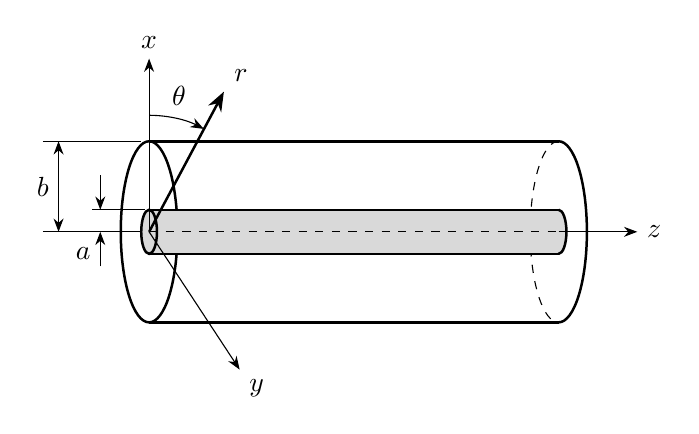
\begin{tikzpicture}[
  >=Stealth,
  font=\normalsize,
  axis/.style={line width=0.4pt},
  curve/.style={line width=0.9pt}
]
  % Outer cylinder (radius b = 1.15)
  \draw[curve] (0,1.15) -- (5.2,1.15);
  \draw[curve] (0,-1.15) -- (5.2,-1.15);
  \draw[curve] (0,0) ellipse (0.36 and 1.15);
  \draw[curve] (5.2,1.15) arc (90:-90:0.36 and 1.15);
  \draw[axis,dashed] (5.2,1.15) arc (90:270:0.36 and 1.15);

  % Inner conductor (radius a = 0.28), shaded
  \fill[black!15] (0,-0.28) -- (5.2,-0.28) arc (-90:90:0.10 and 0.28) -- (0,0.28) arc (90:-90:0.10 and 0.28) -- cycle;
  \draw[curve] (0,0.28) -- (5.2,0.28);
  \draw[curve] (0,-0.28) -- (5.2,-0.28);
  \draw[curve,fill=black!15] (0,0) ellipse (0.10 and 0.28);
  \draw[curve] (5.2,0.28) arc (90:-90:0.10 and 0.28);

  % Coordinate axes
  \draw[axis,->] (0,0) -- (0,2.2) node[above] {$x$};
  \draw[axis,->] (0,0) -- (1.15,-1.75) node[below right] {$y$};
  \draw[axis,dashed] (0,0) -- (5.2,0);
  \draw[axis,->] (5.2,0) -- (6.2,0) node[right] {$z$};

  % Radial vector r and angle theta
  \draw[curve,->] (0,0) -- (0.95,1.78) node[above right] {$r$};
  \draw[axis,->] (0,1.48) arc (90:62:1.48);
  \node at (0.38,1.72) {$\theta$};

  % Radius dimension b
  \draw[axis] (-1.35,1.15) -- (-0.1,1.15);
  \draw[axis] (-1.35,0) -- (-0.1,0);
  \draw[axis,<->] (-1.15,0) -- (-1.15,1.15) node[midway,left] {$b$};

  % Radius dimension a
  \draw[axis] (-0.72,0.28) -- (-0.05,0.28);
  \draw[axis,->] (-0.62,0.72) -- (-0.62,0.28);
  \draw[axis,->] (-0.62,-0.44) -- (-0.62,0);
  \node[left] at (-0.62,-0.28) {$a$};
\end{tikzpicture}
\end{document}
